\documentclass[%
% handout,          % remove the effect of \pause
aspectratio=169,  % default is 4:3 (43), but 16:9 (169) is more popular nowadays
]{beamer}


\usetheme[%
% presenternotes,   % activate presenter notes (PDF comments)
]{LTD}

%%%%%%%%%%%%%%%%% citations%%%%%%%%%%%%%%%%%
\usepackage[square, authoryear]{natbib}
\usepackage{xcolor}


%%%%%%%%%%%%%%%%% media %%%%%%%%%%%%%%%%%
\usepackage{graphicx}
\usepackage[most]{tcolorbox}
\graphicspath{{figures/}}
\usepackage{multimedia}
\newcommand{\includevideo}[2][]{%
	\movie[]%
	{%
		\def\includeargs{#1}
		\ifx\includeargs\empty
			\includegraphics[width=\textwidth,height=\textheight,keepaspectratio]{videos/preview_images/#2.png}%
		\else
			\includegraphics[#1]{videos/preview_images/#2.png}%
		\fi
	}%
	{videos/#2}%
}

%%%%%%%%%%%%%%%%% notes %%%%%%%%%%%%%%%%%
\renewcommand{\note}[1]{%
	{\scriptsize \textcolor{BaseDarkColorA}{\text{#1}}}
}
\usepackage{enumitem}


%%%%%%%%%%%%%%%%% math %%%%%%%%%%%%%%%%%
\usepackage{amssymb}
\usepackage{amscd}
\usepackage{amstext}
\usepackage{amsthm}
\usepackage{amsmath}
\usepackage{physics}
\usepackage{cancel}
\usepackage{bm}
\usepackage{tikz}	

%%% settings for flow charts %%%
\tikzstyle{rect} = [draw, rectangle, fill=white!20, minimum width=3cm, minimum height=1cm,text centered]
\tikzstyle{rect_round} = [draw, rectangle, rounded corners, fill=white!20, minimum width=3cm, minimum height=1cm, text centered]
\tikzstyle{diam} = [draw, diamond,  fill=white!20, minimum width=3cm, minimum height=1cm,text centered]
\tikzstyle{arrow} = [thick,->,>=stealth]
\tikzstyle{line} = [thick]

%%%%%%%%%%%%%%%%% matplotlib %%%%%%%%%%%%%%%%%
\def\mathdefault#1{#1}
\everymath=\expandafter{\the\everymath\displaystyle}
%%   
\ifdefined\pdftexversion\else  % non-pdftex case.
 \usepackage{fontspec}
\fi
\makeatletter\@ifpackageloaded{underscore}{}{\usepackage[strings]{underscore}}\makeatother

\makeatletter
\renewcommand*{\@textcolor}[3]{%
  \protect\leavevmode
  \begingroup
    \color#1{#2}#3%
  \endgroup
}
\makeatother


% load this package to embedded videos in PDF for use with Adobe Acrobat
% don't load it if you want to use Pympress (with videos loaded from the videos directory)
\usepackage[%
autoplay,         % if not enabled, click on videos to play
]{acrobat_embedded_videos}


%%%%%%%%%%%%%%%%%%%%%%%%%%%%%%%%%%
% information about presentation %
%%%%%%%%%%%%%%%%%%%%%%%%%%%%%%%%%%

\title[Short title]{Mathematical formulations for bone remodelling}
\author{Tan Tran}
\date{\today}

% logos on title page
\titlelogos{%
	% \AddLogo{file}{height}
    \AddLogo{TechFakLTD_en.pdf}{9ex}
    \hfill
	\AddLogo{LTD.pdf}{8.2ex}
    \hspace{1.5ex}
    \AddLogo{FAU_white.pdf}{8ex}
}

% logos on regular pages
\logos{%
    % \AddLogo{LTD.pdf}{1.15em}
    % \hspace{-0.75ex}
    \AddLogo{FAU_blue.pdf}{1.2em} 
}

%%%%%%%%%%%%%%
% Begin presentation
%%%%%%%%%%%%%%

\begin{document}

\maketitle

%%%%%%%%%%%%%%%%%%%%%%%%%%%%%%%%%%%%%%%%%%%%%%%%%%%%%%%%%%%
%%%%%%%%%%%%%%%%%%%%%%%%%%%%%%%%%%%%%%%%%%%%%%%%%%%%%%%%%%%

\section{Biochemical model}
\begin{frame}
\begin{figure}
\centering
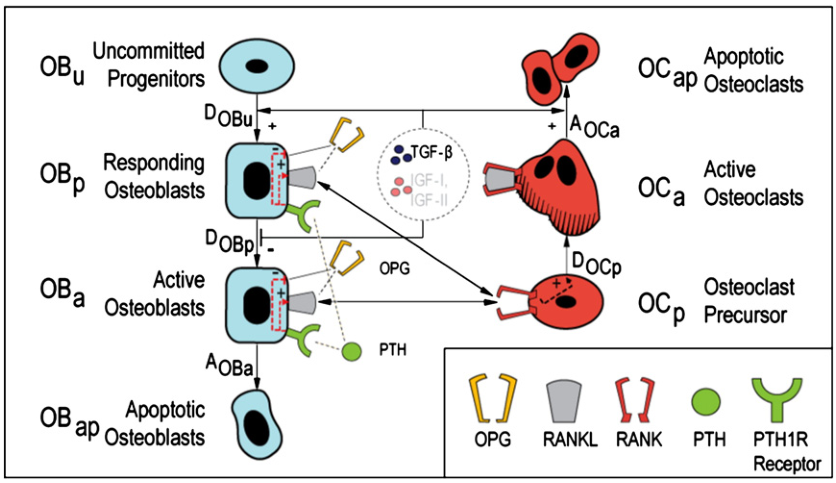
\includegraphics[scale=0.375]{figure_BMU.png}
\caption{Proposed cell population model by \cite{Pivonka.2008} that shows a basic multicellular unit (BMU). The BMU contains osteoblastic cells (OBs) and osteoclastic cells (OC) at different maturation steps including various molecules that influence the differentiation process.}
\end{figure}
\textcolor{gray}{K - RANK, L - RANKL, O - OPG, T - TGF-$\beta$, P - PTH}
\end{frame}
%%%%%%%%%%%%%%%%%%%%%%%%%%%%%%%%%%%%%%%%%%%%%%%%%%%%%%%%%%%

\section{Model by Lemaire(2004)}
\begin{frame}
\textbf{dynamic bone cell population model by \cite{Lemaire.2004}}
\begin{itemize}
	\item[$\bullet$] RANK-RANKL-OPG pathway to regulate OCa formation
	\item [$\bullet$]  PTH injection to regulate OBp, OBa formation
\end{itemize}
\begin{subequations}
	\begin{align}
		& \frac{\text{d} C_\text{OBp}}{\text{d} t} = D_\text{OBp} \cdot \pi_\text{T} - \frac{D_\text{OBa}}{\pi_\text{T}} \cdot C_\text{OBp}\\
		& \frac{\text{d} C_\text{OBa}}{\text{d} t} = \frac{D_\text{OBa}}{\pi_\text{T}} C_\text{OBp} - A_\text{OBa} \cdot C_\text{OBa} \\
		& \frac{\text{d} C_\text{OCa}}{\text{d} t} = D_\text{OCa} \cdot \pi_L(I_\text{L}, I_\text{O}, I_\text{P}) - D_\text{A} \cdot \pi_\text{T}\cdot C_\text{OCa}
	\end{align}
	\label{eq:mode1}
\end{subequations}
\textcolor{gray}{$C_\alpha$ - concentration of $\alpha$, $D_\alpha$ - differentiation rate of $\alpha$, $\pi_\beta$ - proportion of occupied $\beta$ receptors, $A_\alpha$ - apoptosis rate of $\alpha$, $I_\beta$ - injection rate of $\beta$}
\end{frame}
%%%%%%%%%%%%%%%%%%%%%%%%%%%%%%%%%%%%%%%%%%%%%%%%%%%%%%%%%%%

\section*{Model by Pivonka(2008)}
\begin{frame}
\textbf{dynamic bone cell population model by \cite{Pivonka.2008}}
\begin{itemize}
	\item [$\bullet$]  bone volume as new variable
	\item [$\bullet$] RANK-RANKL-OPG pathway expression (by TGF-$\beta$) for OBp, OBa
	\item[$\bullet$] TGF-$\beta$ rate equation depending on bone resorption
\end{itemize}
\begin{subequations}
	\begin{align}
		& \frac{\text{d} C_\text{OBp}}{\text{d} t} =  D_\text{OBu} \cdot \pi_{\text{a,OBu}}^\text{T} (C_\text{T})-  D_\text{OBp}  \cdot \pi_{\text{r,OBp}}^\text{T}(C_\text{T})  \cdot C_\text{OBp}\\
		& \frac{\text{d} C_\text{OBa}}{\text{d} t} =   D_\text{OBp} \cdot  C_\text{OBp} \cdot  \pi_{\text{r,OBp}}^\text{T} (C_\text{T})  \cdot  C_\text{OBp}-  A_\text{OBa}  \cdot C_\text{OBa}\\ 
		& \frac{\text{d} C_\text{OCa}}{\text{d} t} =  D_\text{OCp} \cdot \pi_{\text{a,OCp}}^{\text{L}} (I_\text{O},I_\text{P})-  A_\text{OCa}  \cdot \pi_{\text{a,OCp}}^\text{T}(C_\text{T})  \cdot C_\text{OCa}   \\
		& \frac{\text{d} BV}{\text{d} t} = -k_\text{r} \cdot [C_\text{OCa} - C_\text{OCa}(t_0)] + k_\text{f} \cdot [C_\text{OBa} - C_\text{OBa}(t_0)]
	\end{align}
	\label{eq:model2}
\end{subequations}
\textcolor{gray}{$\pi^\alpha_{\text{a/r}, \beta}$ - activation(a)/repression(r) function of $\alpha$ binding $\beta$, $t_0$ - initial state, $BV$ - bone volume, $k_\text{r/f}$ - resorption/formation rate}
\end{frame}
%%%%%%%%%%%%%%%%%%%%%%%%%%%%%%%%%%%%%%%%%%%%%%%%%%%%%%%%%%%

\section*{Model by Lerebours(2015)}

\subsection{mechanics}
\begin{frame}
\textbf{multiscale mechanobiological femur model by \cite{Lerebours.2016}}
\begin{itemize}
	\item [$\bullet$] material properties on tissue scale based on remodeling process at cellular scale
	\item[$\bullet$] stress/strain on microstructural scale based on macroscopic Euler-Bernoulli beam theory
\end{itemize}
\textbf{stress/strain at tissue level}
\begin{align}
	&\sigma_{11} = \mathbb{C}_{1111} \cdot\varepsilon_{11},~ \sigma_{22} = \mathbb{C}_{1122} \cdot \varepsilon_{11},~ \sigma_{33} = \mathbb{C}_{1133} \cdot \varepsilon_{11} \\
	&\varepsilon_{11} (x_2, x_3) = \varepsilon_1(\mathbb{C}, \mathbf{N}, \mathbf{M}) - \kappa_3(\mathbb{C}, \mathbf{N}, \mathbf{M},t) \cdot x_2 + \kappa_2(\mathbb{C}, \mathbf{N}, \mathbf{M}) \cdot x_3
\end{align}
\textcolor{gray}{$\bm{\sigma}$ - macro stress, $\bm{\varepsilon}$ - macro strain, $\mathbb{C}$ - macro stiffness tensor, $\mathbf{N}$ - normal force, $\mathbf{M}$ - bending moment }
\end{frame}

\begin{frame}
\textbf{stress/strain at cellular level}
\begin{align}
	&\bm{\varepsilon}^m = \mathbb{A}_{bm}(f_bm) :  \bm{\varepsilon},~ \bm{\sigma}^m = \mathbb{B}_{bm}(f_{bm}) :  \bm{\sigma} \\
	&\mathbb{C} = f_{bm} \cdot \mathbb{C}_{bm}^m : \mathbb{A}_{bm} + [1-f_{bm}] \cdot \mathbb{C}_{vas}^m : \mathbb{A}_{vas}
\end{align}
\textbf{strain energy density}
\begin{align}
	& \Psi = \frac{1}{2} \bm{\varepsilon} : \mathbb{C} :  \bm{\varepsilon}  \\
	& \Psi^m = = \frac{1}{2} \bm{\varepsilon}^m : \mathbb{C}^m_{bm} :  \bm{\varepsilon} ^m
\end{align}
\textcolor{gray}{$\bm{\sigma}^m$ - micro stress, $\bm{\varepsilon}^m$ - micro strain, $f_{bm}$ - BV/TV,  $\mathbb{A}_{bm/vas}$ - matrix/vascular strain concentration tensor, $\mathbb{B}_{bm}$ - stress concentration tensor, 
						$\mathbb{C}_{bm/vas}^m$ - matrix/vascular stiffness tensor, $\Psi^{,m}$ - strain energy density}
\end{frame}

\subsection{cell dynamics}
\begin{frame}
\textbf{dynamic bone cell population model by \cite{Lerebours.2016}}
\begin{itemize}
	\item[$\bullet$] incorporation of $\Psi$ into OC actication/repression function
\end{itemize}
\begin{subequations}
	\begin{align}
		& \frac{\text{d} C_\text{OBp}}{\text{d} t} =  D_\text{OBu} \cdot \pi_{\text{a,OBu}}^\text{T}  \cdot C_\text{OBu}(f_{bm}) -  D_\text{OBp}  \cdot \pi_{\text{r,OBp}}^\text{T}  \cdot C_\text{OBp} + \mathcal{P}_\text{OBp} (\Psi)\cdot C_\text{OBp} \\
		& \frac{\text{d} C_\text{OBa}}{\text{d} t} =   D_\text{OBp} \cdot  \pi_{\text{r,OBp}}^\text{T} \cdot  C_\text{OBp} -  A_\text{OBa}  \cdot C_\text{OBa}\\ 
		& \frac{\text{d} C_\text{OCp}}{\text{d} t} =  D_\text{OCu} \cdot \pi_{\text{a,OCu}}^\text{L} (\Psi, \beta_\text{L}) \cdot C_\text{OBu}(f_{bm}) -  D_\text{OCp}  \cdot \pi_{\text{r,OCp}}^\text{L}(\Psi, \beta_\text{L})  \cdot C_\text{OCp}\\
		& \frac{\text{d} C_\text{OCa}}{\text{d} t} =  D_\text{OCp} \cdot \pi_{\text{a,OCp}}^{\text{L}} (\Psi, \beta_\text{L})  \cdot C_\text{OCp}-  A_\text{OCa}   \cdot \pi_{\text{a,OCp}}^\text{T} \cdot C_\text{OCa} \\
	&\frac{\text{d} f_{bm}}{\text{d} t} = -k_\text{r} \cdot C_\text{OCa} + k_\text{f} \cdot C_\text{OBa} 
	\end{align}
\textcolor{gray}{$\mathcal{P}_\text{OBp} $ - proliferation rate of OBp cells, $\beta_L$ - RANKL production rate,}
\label{eq:model3}
\end{subequations}
\end{frame}

\begin{frame}
\textbf{geometrical feedback}
\begin{itemize}
	\item[$\bullet$] $\forall f_{bm} \in [0,1]:$ find $C_\text{OCu}(f_{bm})$ and $C_\text{OBu}(f_{bm})$ s.t 
\end{itemize}
\begin{equation}
	 k_f \cdot \overline{C_\text{OBa}} (C_\text{OBu}(f_{bm}),C_\text{OCu}(f_{bm})) = k_r \cdot  \overline{C_\text{OCa}}(C_\text{OBu}(f_{bm}),C_\text{OCu}(f_{bm})) 
\end{equation}
\textbf{geometrical feedback}
\begin{equation}
	\beta_L (\Psi) = \begin{cases} -\kappa \cdot \mu(\Psi), ~ \text{if} ~ \mu(\Psi) \leq 0\\
		0 ~ \text{else} \end{cases}, 
	\mathcal{P}_\text{OBp} (\Psi) =P_\text{OBp}  +  \begin{cases} 0 , ~ \text{if} ~ \mu(\Psi) \leq 0 \\ 
															P_\text{OBp}  \cdot \lambda \cdot \mu(\Psi) ,~\text{if} ~\mu(\Psi) \in(0,\frac{1}{\lambda}) \\
														P_\text{OBp},  ~\text{else}
											\end{cases}
\label{eq:model3-feedback}
\end{equation}
\textcolor{gray}{$\overline{C_\alpha}$ - steady state concentration of $\alpha$, $\mu$ - normalised $\Psi$ difference, P_$\text{OBp}$ - proliferation term of OBp cells, $\lambda$ - conduction strength}
\end{frame}
%%%%%%%%%%%%%%%%%%%%%%%%%%%%%%%%%%%%%%%%%%%%%%%%%%%%%%%%%%%

\section*{Model by Lavaill(2020)}

\subsection{PK/PD model}
\begin{frame}
\textbf{pharmacokinetics(PK)/pharmacodynamics(PD) model by \cite{Lavaill.2020}}
\begin{itemize}
	\item[$\bullet$] PTH concentration from PK model
	\item[$\bullet$] incorporation of dual PTH action + mech. feedback into cell population model
\end{itemize}
\textbf{PK model}
\begin{itemize}
	\item[$\bullet$] obtain $C_\text{T}$ as external  from following ODEs
\end{itemize}
\begin{subequations}
	\begin{align}
		&\frac{\text{d} D}{\text{d} t} = -k_a \cdot D \cdot F \\
		&\frac{\text{d} C_\text{T}}{\text{d} t} = \frac{F}{V_d} \cdot k_a \cdot D - k_e \cdot C_\text{T} + \beta_\text{T}
	\end{align}
\label{eq:model4-PK}
\end{subequations}
\textcolor{gray}{$D$ - PTH dose, $k_a$ - absorption rate, $F$ - bioavailability, $V_d$ - distribution volume, $k_e$ - elimination rate, $\beta_T$ - PTH production rate}
\end{frame}

\begin{frame}
\textbf{PD model}
\begin{itemize}
	\item[$\bullet$] obtain repressor function $H^{-}_\text{P}(C_{B2})$ to regulate OBa apoptosis from following ODEs
\end{itemize}
\begin{subequations}
	\begin{align}
		&\frac{\text{d} C_{R2}}{\text{d}t} = \beta_{R2} -d_{R2} \cdot H^{+}_{R2} (C_\text{T})\cdot C_{R2} \\
		&\frac{\text{d}C_{pC}}{\text{d}t} = \beta_{pC} \cdot H^{+}_{pC} (C_\text{T})  - d_{pC} \cdot C_{pC} \\ 
		&  \frac{\text{d} C_{B2}}{\text{d}t} = \beta_{B2} \cdot C_{R2} \cdot C_{pC} - d_{B2} \cdot C_{B2}
	\end{align}
\label{eq:model4-PD}
\end{subequations}
\textcolor{gray}{$R2$ - Runx2, $pC$ - pCREB, $B2$ - Bcl-2, $\beta$ - production rate, $d$ - degradation rate, $H$ - regulation function }
\end{frame}

\subsection{cell dynamics}
\begin{frame}
\textbf{dynamic cell population model by \cite{Lavaill.2020}}
\begin{itemize}
	\item[$\bullet$] catabolic PTH action in $\pi_{\text{a,OCp}}^{\text{L}} $, anabolic PTH action in $A_\text{OBa}$
	\item{$\bullet$} $\Psi$ based on \cite{Lerebours.2016}
	\item[$\bullet$]  geometrical and mechanical feedback from (\ref{eq:model3-feedback})
\end{itemize}
\begin{subequations}
	\begin{align}
		& \frac{\text{d} C_\text{OBp}}{\text{d} t} =  D_\text{OBu} \cdot \pi_{\text{a,OBu}}^\text{T} \cdot C_\text{OBu} -  D_\text{OBp}  \cdot \pi_{\text{r,OBp}}^\text{T} \cdot C_\text{OBp} + \mathcal{P}_\text{OBp} \cdot C_\text{OBp}  \\
		& \frac{\text{d} C_\text{OBa}}{\text{d} t} =   D_\text{OBp}  \cdot  \pi_{\text{r,OBp}}^\text{T} \cdot  C_\text{OBp}-  A_\text{OBa} \cdot H^{-}_\text{P} \cdot C_\text{OBa}\\ 
		& \frac{\text{d} C_\text{OCa}}{\text{d} t} =  D_\text{OCp} \cdot \pi_{\text{a,OCp}}^{\text{L}} \cdot C_\text{OCp} -  A_\text{OCa}   \cdot \pi_{\text{a,OCp}}^\text{T} \cdot C_\text{OCa}  \\
		&\frac{\text{d} f_{bm}}{\text{d} t} = -k_\text{r} \cdot C_\text{OCa} + k_\text{f} \cdot C_\text{OBa} 
	\end{align}
\label{eq:model4}
\end{subequations}
\end{frame}
%%%%%%%%%%%%%%%%%%%%%%%%%%%%%%%%%%%%%%%%%%%%%%%%%%%%%%%%%%%

\section*{Model by Sansalone(2020)}

\subsection{mechanics}
\begin{frame}
\textbf{continuum mechanical model for bone turnover by \cite{Sansalone.2021}}
\begin{itemize}
\item[$\bullet$] bone turnover: resorption $\rightarrow$ formation $\rightarrow$ mineralisation
\item[$\bullet$] three distinct phases: porosity (p), mineralised bone (m), unmineralised bone (u)
\end{itemize}
\textbf{kinematics}
\begin{subequations}
	\begin{align}
		&\dot{f}_u = \dot{f}_u^\text{OB} + \dot{f}_u^\text{OC} + \dot{f}_u^{\chi} \\
		&\dot{f}_m = \dot{f}_m^\text{OC} + \dot{f}_m^{\chi} \\
		&\dot{f}_p = 1 - \dot{f}_u - \dot{f}_m
	\end{align}
\end{subequations}
\textcolor{gray}{$\dot{(*)} = \frac{\text{d(*)}}{\text{d}t}$, OB - formation mechanism, OC - resorption mechanism, $\chi$ - mineralisation mechanism, $f_\alpha^\beta$ - vol. fraction of phase $\alpha$ due to mechanism $\beta$}
\end{frame}

\begin{frame}
\textbf{balance equations}
\begin{subequations}
	\begin{align}
		& \text{div} (\bm{\sigma}) + \mathbf{b} = \mathbf{0} ~\text{in} ~ \mathcal{B}_0 ~ \text{with} ~\bm{\sigma} \cdot \mathbf{n} = \mathbf{t}  ~\text{in} ~\partial \mathcal{B}_0 \\
		& \overset{i}{\mathbf{T}} + \overset{o}{\mathbf{T}} = 0~\text{in} ~ \mathcal{B}_0 \\
		& \overset{i}{\lambda}^\text{OB}_u + \overset{i}{\lambda}^\text{OB}_u = 0 ~\text{in} ~ \mathcal{B}_0\\
		& \overset{i}{\lambda}^\text{OC}_u + \overset{i}{\lambda}^\text{OC}_u = 0 ~\text{in} ~ \mathcal{B}_0\\
		& \overset{i}{\lambda}^\text{OB}_m + \overset{i}{\lambda}^\text{OB}_m = 0 ~\text{in} ~ \mathcal{B}_0\\
		& [\overset{i}{\lambda}^{\chi}_m-\overset{i}{\lambda}^{\chi}_u] +  [\overset{o}{\lambda}^{\chi}_m-\overset{o}{\lambda}^{\chi}_u] = 0 ~\text{in} ~ \mathcal{B}_0
	\end{align}
	\label{eq:model5-balance}
\end{subequations}
\textcolor{gray}{$\mathbf{b}$ - body force, $\mathbf{t}$ - surface traction, $\mathbf{n}$ - surface normal, $\mathcal{B}_0$ - reference body, $\mathbf{T}$ - rotary remodelling tensor, $\lambda_\alpha^\beta$ - remodelling force in phase $\alpha$ due to mechanism $\beta$, $^{i/o}$ - inner/outer}
\end{frame}

\subsection{evolution laws}
\begin{frame}
\textbf{temporal change of bone phases}
\begin{subequations}
	\begin{align}
		& \dot{f}_u^\text{OB} = \frac{C_\text{OB}}{\overline{d}_u^\text{OB}} \cdot [\alpha_u^\text{OB} \cdot S_V - \lambda^\text{mech}_u(\mathbb{C}, \varepsilon) - \lambda^\text{chem}_u(\mu_p, \mu_m, \mu_u) ] \\
		&\dot{f}_u^\text{OC} = \frac{C_\text{OC}}{\overline{d}_u^\text{OC}} \cdot [\alpha_u^\text{OC} \cdot f_u \cdot (f_p - f_p^\text{min}) - \lambda^\text{mech}_u(\mathbb{C}, \varepsilon) - \lambda^\text{chem}_u(\mu_p, \mu_m, \mu_u)] \\
		& \dot{f}_m^\text{OC} =  \frac{C_\text{OC}}{\overline{d}_m^\text{OC}} \cdot [\alpha_m^\text{OC} \cdot f_m \cdot (f_p - f_p^\text{min}) - \lambda^\text{mech}_m(\mathbb{C}, \varepsilon) - \lambda^\text{chem}_m (\mu_p, \mu_m, \mu_u)] \\
		& \dot{f}_m^\chi = \frac{f_u\cdot f_m}{\overline{d}^\chi} \cdot [(\overset{o}{\lambda}^{\chi}_m-\overset{o}{\lambda}^{\chi}_u) - \Delta  \lambda^\text{mech}(\mathbb{C}, \varepsilon) - \Delta  \lambda^\text{chem}(\mu_p, \mu_m, \mu_u) ]
	\end{align}
\end{subequations}
\textcolor{gray}{$\overline{d}$ - turnover ressistance, $\alpha$ - unit stimuli, $S_V$ - specific surface, $\lambda^\text{mech/chem}_{u/m}$ - generalised mech./chem. turnover force in phase $u/m$ }
\end{frame}
%%%%%%%%%%%%%%%%%%%%%%%%%%%%%%%%%%%%%%%%%%%%%%%%%%%%%%%%%%%

\section{Model by Martonova(2023)}
\subsection{two-state model}
\begin{frame}
\textbf{two-state receptor ligand binding model for PTH by \cite{Martonova.2023}}
\begin{itemize}
	\item[$\bullet$] PTH1R regulates skeletal development and transduces stimuli from PTH
	\item[$\bullet$] modelling activation of PTH1R
\end{itemize}
\begin{equation}
	\begin{bmatrix}
		\dot{r}_a \\ \dot{c}_a \\ \dot{c}_i
	\end{bmatrix} =
	\begin{bmatrix}
		-k_1 -k_r \cdot C_\text{P} & k_{-r} & 0 & k_{-1} \\
		k_r \cdot C_\text{P}  & -k_2-k_{-r} & k_{-2} & 0 \\
		0 & k_2 & -k_{-2} -k_{-d} & k_d \cdot C_\text{P} 
	\end{bmatrix} \cdot
	\begin{bmatrix}
		r_a \\ c_a \\ c_i \\ 1-(r_a+c_a+c_i)
		\end{bmatrix}
	\label{eq:model6}
\end{equation}
\textcolor{gray}{$r_a$ - active receptor fraction, $c_{i/a}$ - inactive/active ligand-receptor complex fraction, $k_i$ - kinematic parameters }
\end{frame}

\begin{frame}
\textbf{PTH concentration}
\begin{itemize}
	\item[$\bullet$]Obtain separate $C_\text{P}$ values due to internal secretion and external drug dosing
\end{itemize}
\begin{equation}
	C_\text{P} = \begin{cases}
		\gamma_1 ~ \text{if} ~ (n-1) \cdot T \leq t \leq (n-1)\cdot T + \tau_1 \\
		\gamma_0 ~ \text{if} ~ (n-1) \cdot T + \tau_1 \leq t \leq (n-1) \cdot T + \tau_1 + \tau_0
	\end{cases}
\end{equation}
\textbf{cellular responsiveness} $\alpha_R$
\begin{align}
	&\alpha_R = \frac{\alpha_T}{\alpha_{T_\text{step}}} \cdot \frac{\alpha_T}{T} \\
	& \alpha_T = \int_0^{T} [\alpha(r_a, c_a, c_1, r_i) -\alpha_0] dt ~\text{with} ~ T = \tau_0+\tau_1
\end{align}
\textcolor{gray}{$\gamma_{0/1}$ - PTH concentration due to tonic/pulsatile glandular secretion, $\tau_{0,1}$ - off-/on-phase, $n$ - pulses, $\alpha_{T_\text{step}}$ - integrated activity, $\alpha$ - scaled activity}
\end{frame}

\subsection{optimal cellular responsiveness}
\begin{frame}
\textbf{Predict optimal pulsatile pattern}
\begin{equation}
	\underset{\gamma_1, \tau_1}{\text{argmin}} ~ [\alpha_R(C_\text{P}^{gl} - \alpha_R^{ref})]^2
\end{equation}
\textbf{Predict optimal dosing pattern}
\begin{equation}
	\underset{D}{\text{argmin}} ~ [\alpha_R^\text{inj}(D) -( \alpha_R^{ref}-\alpha_R^{ill})]^2
\end{equation}
\textcolor{gray}{$C_\text{P}^{gl}$ - plasma PTH concentration, $\alpha_R^{ref/ill}$ healthy/unhealthy cellular responsiveness}
\end{frame}

%%%%%%%%%%%%%%%%
\section*{References}%
%%%%%%%%%%%%%%%%
\begin{frame}[allowframebreaks]
\bibliographystyle{apalike}
   \bibliography{bibfile}
\end{frame}

\end{document}
